% ===============================
\section{Selected fund managers}\label{sec:selected-fund-managers}

    I consider a list of 20 GPs and 20 LPs, selected by fund size and reported in table~\ref{tab:selected_funds}.

    \begin{sidewaystable}[ht]
    \centering
    \caption{Top 20 Private Equity GPs and LPs by Fund Size or Commitment (USD mn)}
    \begin{tabular}{l r | l r}
    \hline
    \textbf{GP} & \textbf{Fund Size} & \textbf{LP} & \textbf{Commitment} \\
    \hline
    TPG & 57,088.5 & California Public Employees' Retirement System & 29,685.33 \\
    The Carlyle Group & 53,275.79 & CPP Investments & 25,130.54 \\
    Apollo Global Management & 52,034 & California State Teachers' Retirement System & 22,637.9 \\
    Blackstone & 46,950 & Washington State Investment Board & 16,853.35 \\
    CVC Capital Partners & 38,355.47 & Oregon Public Employees Retirement Fund & 16,093.9 \\
    Apax Partners & 35,544.61 & New York State Common Retirement Fund & 15,128.15 \\
    Goldman Sachs Asset Management & 30,550 & Teacher Retirement System of Texas & 14,248.47 \\
    Bain Capital & 29,507 & Florida State Board of Administration & 11,212.6 \\
    Kohlberg Kravis Roberts & 28,572.18 & Hamilton Lane & 9,833.73 \\
    Advent International & 27,559.44 & Pennsylvania Public School Employees' Retirement System & 8,414.04 \\
    Permira & 25,125.9 & Michigan Department of Treasury & 8,283.78 \\
    Silver Lake & 23,300 & State of Wisconsin Investment Board & 6,602.43 \\
    Providence Equity Partners & 22,808 & Massachusetts Pension Reserves Investment Management Board & 6,277.31 \\
    Madison Dearborn Partners & 22,163 & Teachers Retirement System of Georgia & 5,321.97 \\
    EQT & 19,486.98 & Teachers' Retirement System of the State of Illinois & 5,215.23 \\
    Nordic Capital & 16,014.86 & State Teachers Retirement System of Ohio & 5,204.57 \\
    Welsh, Carson, Anderson \& Stowe & 15,386.7 & Los Angeles County Employees' Retirement Association & 5,058.98 \\
    Leonard Green \& Partners & 15,007 & New York State Teachers' Retirement System & 4,736.66 \\
    Charterhouse Capital Partners & 14,468.42 & Maryland State Retirement and Pension System & 4,675 \\
    Onex & 13,810 & Minnesota State Board of Investment & 4,596.94 \\
    \hline
    \end{tabular}
    \label{tab:selected_funds}
    \end{sidewaystable}

    For each of them, all the investor documents that contain the fund name are obtained from Preqin, and stored for LLM processing.
    \begin{table}[ht]
        \centering
        \caption{Number of retrieved documents}
        \resizebox{\textwidth}{!}{%
        \begin{tabular}{l r}
            \hline
            \textbf{LP} & \textbf{Number of documents} \\
            \hline
            California Public Employees' Retirement System & 359 \\
            CPP Investments & 103 \\
            California State Teachers' Retirement System & 142 \\
            Washington State Investment Board & 84 \\
            Oregon Public Employees Retirement Fund & 114 \\
            New York State Common Retirement Fund & 139 \\
            Teacher Retirement System of Texas & 127 \\
            Florida State Board of Administration & 247 \\
            Hamilton Lane & 1571 \\
            Pennsylvania Public School Employees' Retirement System & 71 \\
            Michigan Department of Treasury & 73 \\
            State of Wisconsin Investment Board & 147 \\
            Massachusetts Pension Reserves Investment Management Board & 56 \\
            Teachers Retirement System of Georgia & 53 \\
            Teachers' Retirement System of the State of Illinois & 246 \\
            State Teachers Retirement System of Ohio & 137 \\
            Los Angeles County Employees' Retirement Association & 209 \\
            New York State Teachers' Retirement System & 84 \\
            Maryland State Retirement and Pension System & 122 \\
            Minnesota State Board of Investment & 96 \\
            \hline
            Total & 4180 \\
            \hline \\
            \hline
            \textbf{GP} & \textbf{Number of documents} \\
            \hline
            TPG & 810 \\
            The Carlyle Group & 455 \\
            Apollo Global Management & 687 \\
            Blackstone & 1403 \\
            CVC Capital Partners & 1014 \\
            Apax Partners & 800 \\
            Goldman Sachs Asset Management & 947 \\
            Bain Capital & 1241 \\
            Kohlberg Kravis Roberts & 485 \\
            Advent International & 757 \\
            Permira & 903 \\
            Silver Lake & 908 \\
            Providence Equity Partners & 283 \\
            Madison Dearborn Partners & 89 \\
            EQT & 2719 \\
            Nordic Capital & 388 \\
            Welsh, Carson, Anderson \& Stowe & 617 \\
            Leonard Green \& Partners & 425 \\
            Charterhouse Capital Partners & 140 \\
            Onex & 895 \\
            \hline
            Total & 15966 \\
            \hline
        \end{tabular}
        }
        \label{tab:num_of_docs}
    \end{table}
    Finally, for the 20 GPs, the cash flows of the years 2014--2024 for the funds they manage are also obtained.
    The cash flows database contains, complemented by fund metadata

\section{LLM and Computational Setup}\label{sec:llm-and-computational-setup}
    When working with large language models (LLMs), the choice of hardware is crucial, as even modestly sized models require substantial GPU resources.
    Insufficient computational power can limit access to state-of-the-art models and reduce experimental flexibility.
    For this analysis, I employ \href{https://www.deepseek.com/}{\underline{DeepSeek-r1}}, an open-weights, reasoning-focused, LLM introduced by the DeepSeek AI research team in late 2024 and officially released in January 2025.
    The model quickly became a disruptive force in the AI landscape, even contributing to a significant selloff in Nvidia’s stock by demonstrating strong performance on relatively modest hardware.
    In particular, I rely on the compact version, \textit{DeepSeek-r1:8B} (8 billion parameters), which balances computational efficiency with high reasoning capabilities (see~\ref{lst:deepseek-r1}).

    \begin{center}
        \begin{minipage}{0.85\linewidth}
            \begin{lstlisting}[style = cmd,label={lst:deepseek-r1}]
                Model
                    architecture        qwen3
                    parameters          8.2B
                    context length      131072
                    embedding length    4096
                    quantization        Q4_K_M

                Capabilities
                    completion
                    thinking

                Parameters
                    stop           "<｜begin▁of▁sentence｜>"
                    stop           "<｜end▁of▁sentence｜>"
                    stop           "<｜User｜>"
                    stop           "<｜Assistant｜>"
                    temperature    0.6
                    top_p          0.95

                License
                    MIT License
                    Copyright (c) 2023 DeepSeek
            \end{lstlisting}
        \end{minipage}
    \end{center}

    The model is deployed locally on the hardware of choice, an MSI GS65 laptop mounting an NVIDIA GeForce GTX~1070 GPU with 8\,GB of VRAM (CUDA~12.8), through \href{https://ollama.com/}{\underline{Ollama}}, a lightweight framework that lets you run large language models locally on your machine with simple commands and efficient resource management.
    Particularly, \textit{Ollama} exposes an API through which the locally installed model can be queried by sending requests containing a prompt expressed in natural language.
    For this analysis, the prompt consists in textual content from the investor documents, and instructions on how to process it (depicted in Fig. \ref{fig:workflow}).

    \begin{figure}
        \centering
        \label{fig:workflow}
        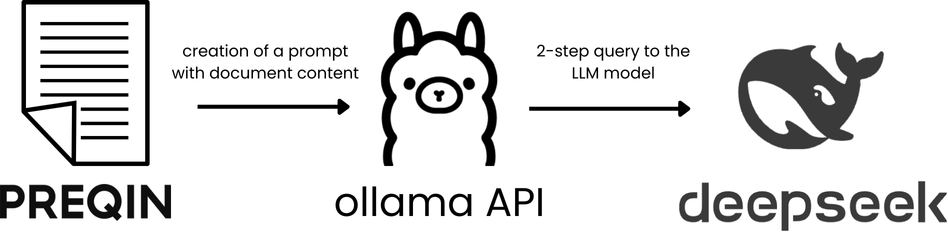
\includegraphics[width=0.85\linewidth]{img/workflow}
        \caption{Workflow schematic with main components.}
    \end{figure}